% !TeX root = ../main.tex
% Add the above to each chapter to make compiling the PDF easier in some editors.
\chapter{Application: Apache Flink Benchmark}\label{chapter:benchmark}

Having implemented a tool for time series generation, we will now look at an application of these time-series. There are many possible applications, a good example is using the time series to simulate load on a system for benchmarking purposes. Sticking with the distributed systems theme started in Chapter \ref{chapter:hmm-dist} with the HMM implementation in Apache Spark, we will look at Apache Flink. Flink is among other things a good batch processing tool and it has an easy API for submitting these batch jobs. This makes it a great candidate for benchmarking using the generated time series. 

\section{Apache Flink}

Apache Flink is an open-source framework for processing both streaming and batch data. Applications of Flink include real-time analytics, historic data processing and various task in the machine learning and graph analysis field. Flink's paradigm is to use data-stream processing as the underlying model for all tasks. This includes batch processing, which in Flink is considered just a special case of stream processing, where the stream is finite. 

Flink is a cluster computing platform. One Flink cluster consists of multiple parts: the client, the Job Manager and one or more Task Managers. The client turns a program into a dataflow graph and submits it to the Job Manager. The Job Manager is responsible for coordinating the execution of this dataflow graph. It schedules jobs for the Task Managers, which do the actual computation and report the results back to the Job Manager \parencite{carbone2015apache}.

\section{Flink Job: Pi Estimation}

The idea is to benchmark Flink by submitting batch jobs to it according to our time series. For this we need a job that is sufficiently resource intensify to be noticeable. The official Flink batch processing examples provide a good candidate: a pi estimation job. Flink jobs are written in Java and the code for this job can be found at \parencite{flinkpiestim}. 

The idea is tho pick random points by drawing x and y such that $0 < x, y < 1$. Then we check wether or not these points are in the unit circle with $x^2 + y^2 < 1$. We know that the area of the first quadrant segment of the unit circle is $\frac{\pi}{4}$ while the area of the square that the points all fall into is 1. Thus, we know that the fraction of the samples that fall in the unit-circle times 4 will approximate $\pi$.

The number of samples to consider can be specified via a parameter. The more samples the better the estimate. Using this parameter we can control how much compute we want our job to consume. 

\section{Benchmarking}

From the time-series generation tool we receive a set of discrete time points each with a value. This is not great since real world tasks do not arrive at whole seconds. We address this by considering normal distributions each with its mean at one of the time points. Then We draw from these normal distributions a number of times according to the value of the time series at that point. Figure \ref{fig:normal-dists} visualizes these normal distributions.

\begin{figure}
   \centering
   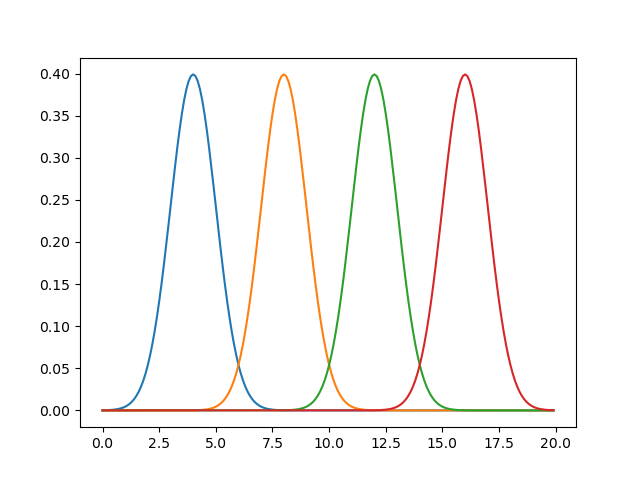
\includegraphics[scale=0.70]{figures/normal-dists.png}
\caption{Normal Distributions}    
\label{fig:normal-dists}
\end{figure}

At this point we have a sequence of absolute time points. For the benchmarking now we simply start a timer and whenever we hit one of these time points we submit a job. The script performing the benchmark goes one step further. Since we can specify the amount of compute a job takes with a parameter, we can simulate different kinds of jobs. The current scripts considers two generated time-series: one modeling an easy and one modeling an expensive job \parencite{flinktest}.

While submitting jobs according to the schedule, at each full second we pull metrics from both the Flink Task Manager and the Job Manager. Using this we can monitor how Flink handles the simulated work load.

\section{Flink API}

There are multiple ways to interface with Flink. The most convenient for this kind of application is the REST API. 

The first relevant endpoint is \texttt{/jars}. Jobs in Flink are Java programs and therefore distributed as jars. First we build the pi estimation code into such a jar. Then Flink needs to know about this job. This can be achieved by submitting the jar file via a POST request to the endpoint \texttt{/jars/upload}. The jar is assigned an id, which is contained in the response of the upload request. All of this only has to happened once. 

To run a submitted job we can submit a POST request to \texttt{/jars/:jarid/run}. The \texttt{jarid} being the id received at upload. Using the query parameter \texttt{programArgs} we can submit arguments to the job. In the Pi estimation case the number of samples. 

Because of Flink's architecture there are two places that we are interested in collecting metrics from: the Job Manger and the Task Manager. The respective endpoints for these are \texttt{/jobmanager/metrics} and \texttt{/taskmanagers/metrics}. The two endpoints behave exactly the same. Making a GET request without a query parameter returns a list of available metrics. To receive their values append the ids of the desired metrics via the "get" query parameter. This will return the metric values in a JSON format \parencite{flinkrest}.

\section{Results}

\begin{figure}
   \centering
   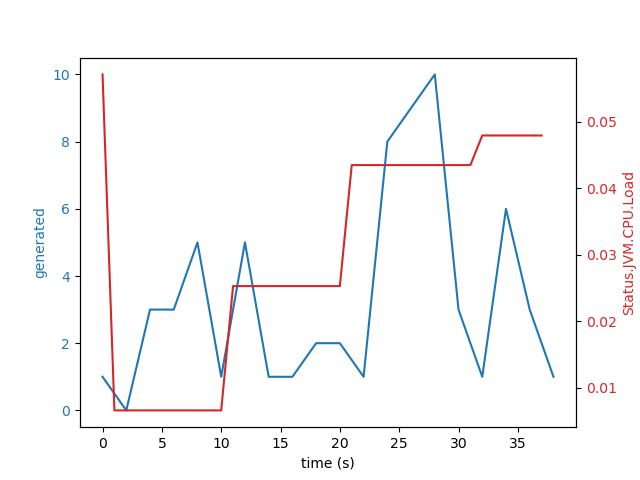
\includegraphics[scale=0.70]{figures/cpu-load.png}
\caption{CPU Load}    
\label{fig:bench-cpu}
\end{figure}

\begin{figure}
   \centering
   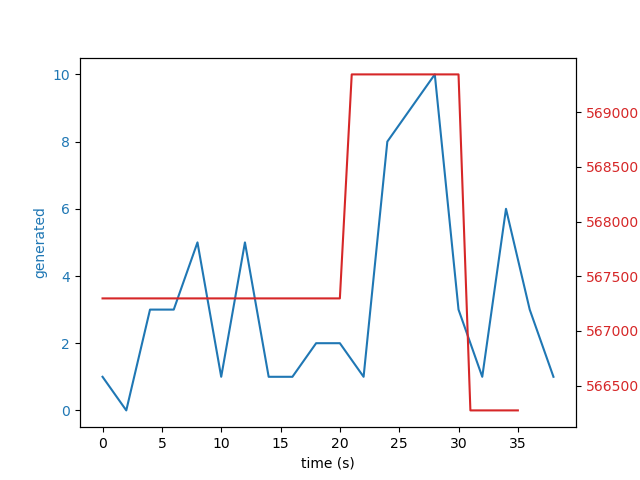
\includegraphics[scale=0.70]{figures/memory-used.png}
\caption{Memory Used}    
\label{fig:bench-memory}
\end{figure}

\begin{figure}
   \centering
   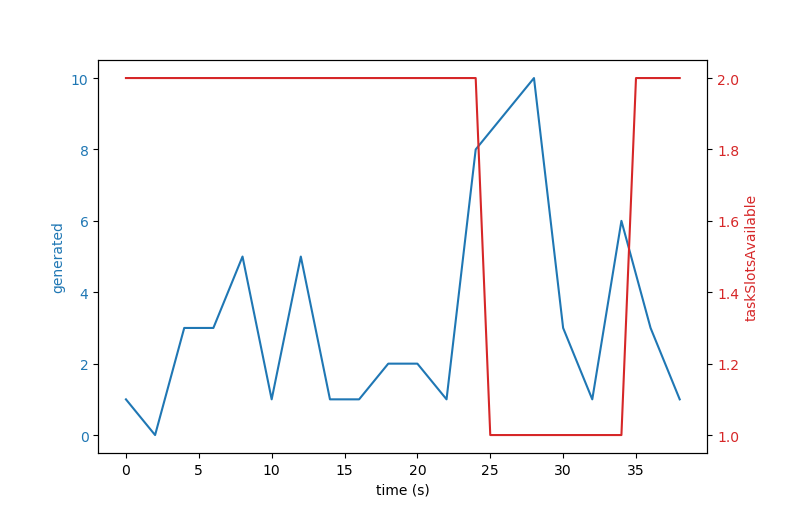
\includegraphics[scale=0.60]{figures/task-slots.png}
\caption{Task Slots}    
\label{fig:bench-taks}
\end{figure}

\begin{figure}
   \centering
   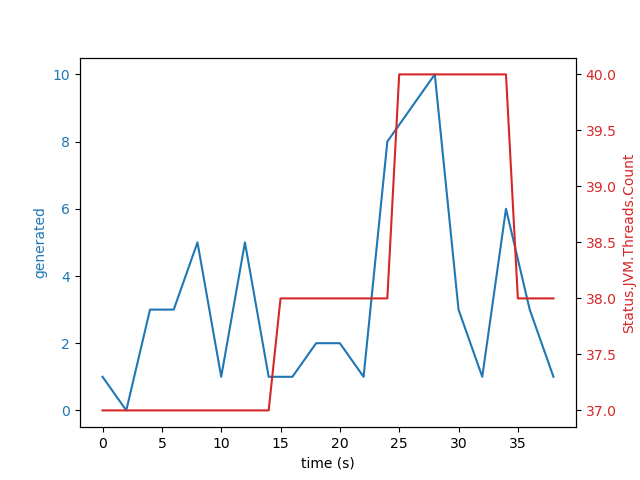
\includegraphics[scale=0.70]{figures/threads.png}
\caption{Threads}    
\label{fig:bench-threads}
\end{figure}

Figure \ref{fig:bench-cpu} through \ref{fig:bench-threads} show graphs of some of the metrics overlaid with the time series that generated them. Note that in this case there is only one time-series that is scheduling jobs of one kind. The graphs quickly become unreadable when adding more time series. 

All of these were generated on Windows 10 using the Docker version of Flink \parencite{flinkdocker}.

The result are as expected: the metrics for CPU, Memory, and Threads are related to the generated time-series. When many jobs get submitted their metrics go up as well. \texttt{taskSlotsAvailable} on the other hand has an inverse relationship. This also makes sense: as many jobs are being worked on the task slots are full. 